\documentclass[14pt]{extarticle}
\usepackage[utf8]{inputenc}
\usepackage[a4paper, margin=1in]{geometry}
\usepackage{tikz}
\usepackage{color}
\usepackage{subfiles}
\usepackage[T1]{fontenc}
\usepackage{titlepic}
\usepackage{amssymb}
\usepackage{graphicx}
\usepackage{caption}
\usepackage{subcaption}
\usepackage{listings}
\usepackage{minted}
\usepackage[section]{placeins}

\title{\Huge{\textcolor{blue}{TCP Reset Attack on Video Streaming}} \\ ~\\
        % \Huge{DRAFT}
        \LARGE{Design Report} \\ ~ \\ ~ \\ }
\author{Abdullah Al Ishtiaq \\
        \textbf{Student Id. : 1505080}}
\date{\today}


\begin{document}

\maketitle

\vspace{1cm}

\begin{figure}[h!]
\centering
    
\includegraphics[width = 0.25\textwidth]{Pictures/logoBUET.png}
\end{figure}
\begin{center}
\vspace{.5cm}

\Large{Department of Computer Science and Engineering \\
    Bangladesh University of Engineering and Technology \\
    (BUET) \\
    Dhaka - 1000 }

\end{center}

\newpage
%==================================================================

\tableofcontents
\newpage

\listoffigures
\newpage

%==================================================================

\section{Introduction}
    The Transmission Control Protocol (TCP) is a core protocol of the Internet Protocol Suite. It is one of the 2 main transport layer protocols which sit on top of the IP layer. TCP provides reliable, ordered and error-checked host-to-host communication services for applications. It is considered a stateless protocol suite because each client connection is newly made without considering whether a previous connection had been established or not. \\
    Although TCP is widely used in major internet applications, it introduces a few vulnerabilities too. The most common of these vulnerabilities are: Denial of Service (DOS), Connection Hijacking, TCP Veto, TCP Reset attack etc.

\section{TCP Reset Attack on Video Streaming}
    TCP reset attack on video streaming applications does not target the protocol's typical method of closing a connection which uses a 4-way handshake method. Rather it uses the protocol's method of immediately terminating an unwanted, unexpected or erroneous connection. From the specifications of Transmission Control Protocol (TCP) given in RFC-0793 (September 1981) we quote, "Reset (RST) must be sent whenever a segment arrives which apparently is not intended for the current connection". It is an important property of TCP for ensuring robustness, but at the same time it has opened up a scope of exploitation. \\ 
    In TCP reset attack on video streaming, an attacker forges a spoofed RST packet that pretends to be one coming from the original video streaming server. As a result the victim immediately closes the TCP connection and goes to CLOSED state. In addition to that, upon receiving additional packets from the original server, the victim itself sends RST packet to the server terminating the connection at the remote end. In this way the attacker can successfully disrupt video streaming on its victim's machine.

\section{Strategy}
   
    The  strategy of our attack can be described in 3 steps. Those are:
    \begin{enumerate}
      \item First we need to find out the IP address of either the victim machine or the video server.
      \item Then we have to sniff packets in the network to discover the other IP address, the TCP port numbers and the correct sequence number.
      \item Finally we forge a TCP packet with correct IP addresses, TCP Port numbers and sequence number and with RST bit set and send it to the victim machine.
    \end{enumerate}
    
     \label{sec:strategy}
    
    \textsl{Here one important aspect needs to be discussed. We can also perform the attack by sending forged RST packets to the video streaming server, but chances are that it will be self harmful as the server may block the attacker's IP address. So instead of doing so, we are going to send the forged packets to the victim machine.}  \\
    \textsl{Another important note is that we must send the packet with haste as the sequence number in the forged RST packet must be within victim's window to  be effective. Otherwise it will be discarded without any impact on the connection.}
  

\section{Timing Diagrams}
    
    \begin{figure}
    	\centering
    	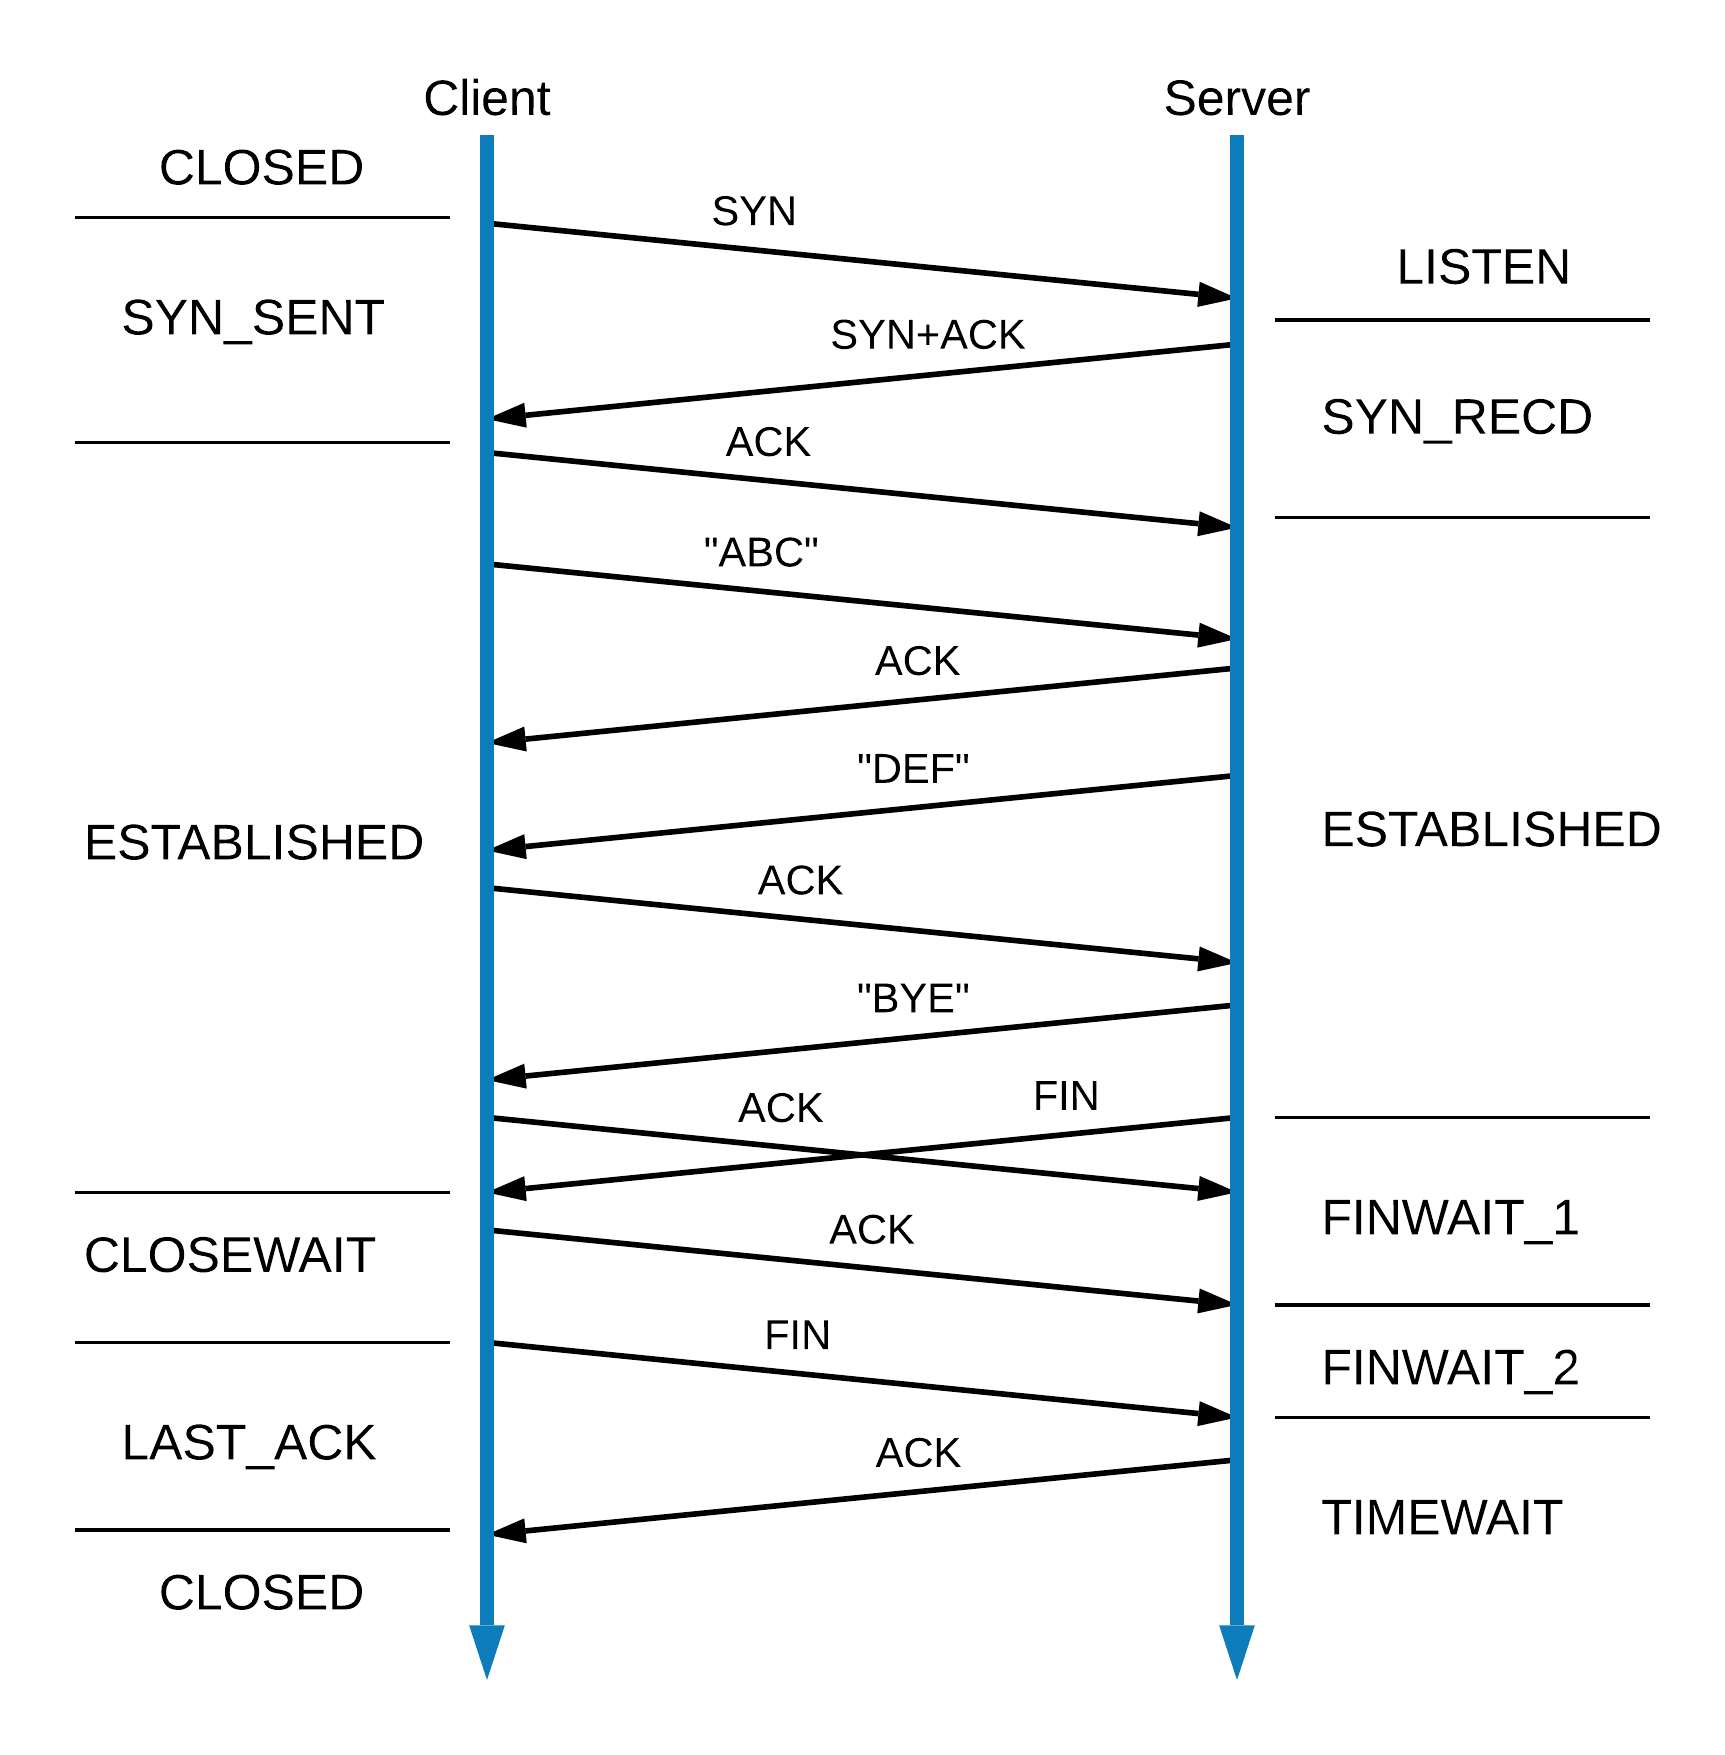
\includegraphics[width=.95\textwidth]{Pictures/TCP_Timing_Diagram.png}
    	\caption{TCP Timing Diagram}
    	\label{fig:TCP_Tim}
    \end{figure}
    
    In figure \ref{fig:TCP_Tim}, the timing diagram of typical communication for video streaming between the streaming server and victim is shown. Here connection can be closed by either of the parties and in both cases a 4-way handshake will occur. 
    
    \begin{figure}
    	\centering
    	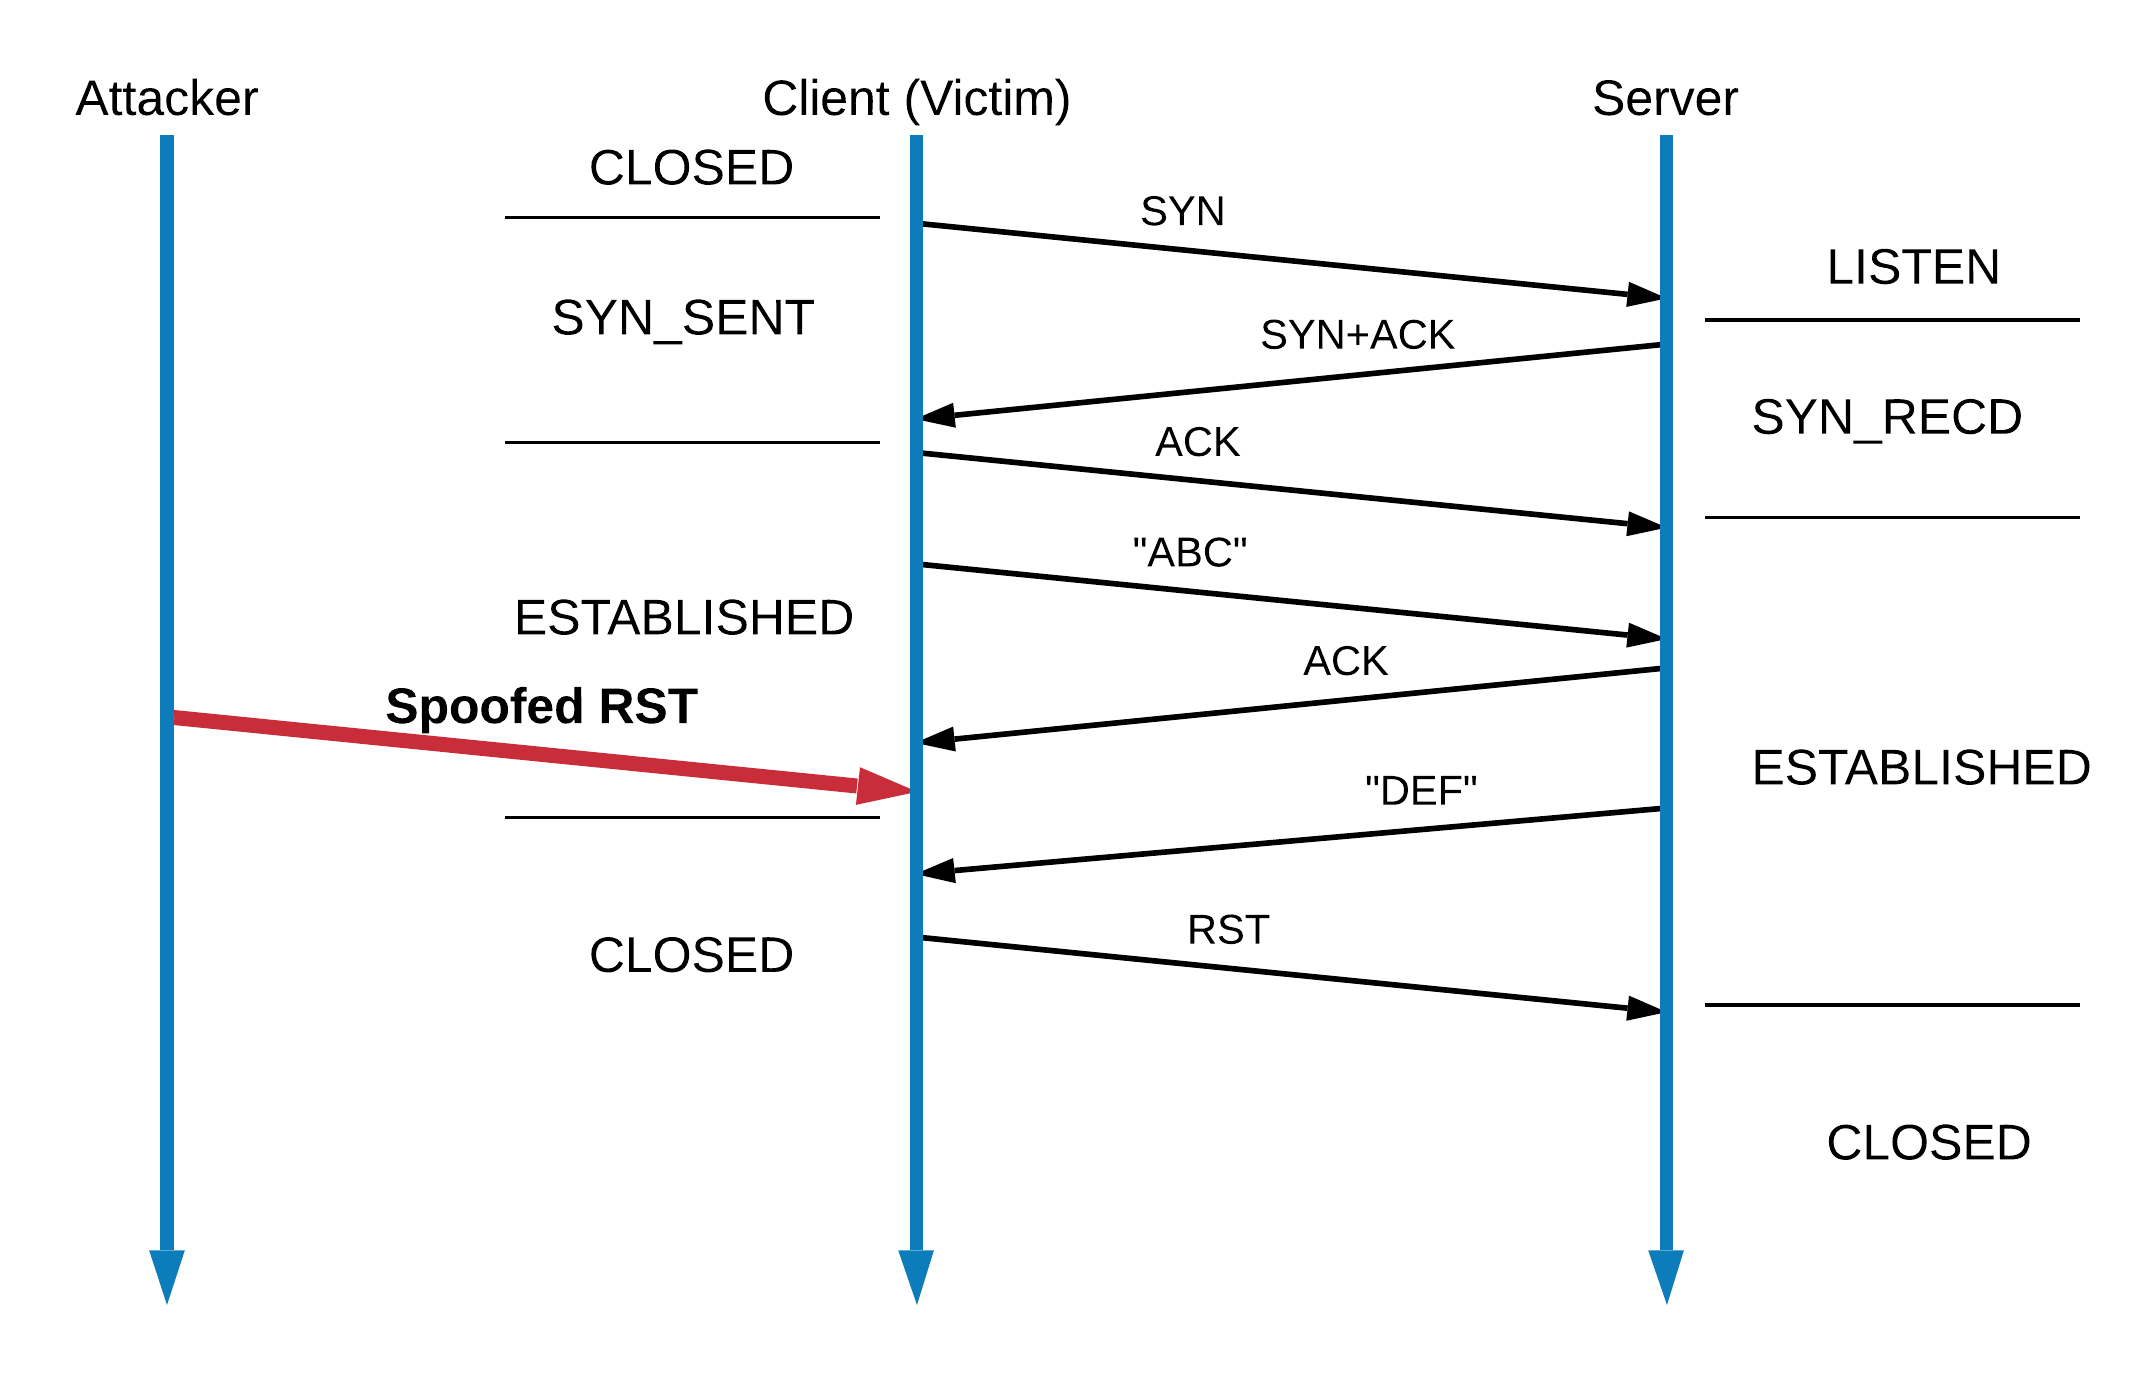
\includegraphics[width=.95\textwidth]{Pictures/TCP_RST_Timing_Diagram.png}
    	\caption{TCP Reset Attack Timing Diagram} 
    	\label{fig:RST_Attack_Tim}
    \end{figure}
    
    We will perform the TCP reset attack by sending forged RST packet from the attacker machine. The timing diagram of the attack is shown in figure \ref{fig:RST_Attack_Tim}. In this case the victim will assume the video server has unexpectedly terminated the TCP connection, and upon receiving additional messages it will send RST back to the server. Finally the server will also close the connection receiving the RST packet. \\ 
    These timing diagrams are drawn according to the specifications provided in RFC-0793.
    
\section{Packet Details}
    \begin{figure}
    	\centering
    	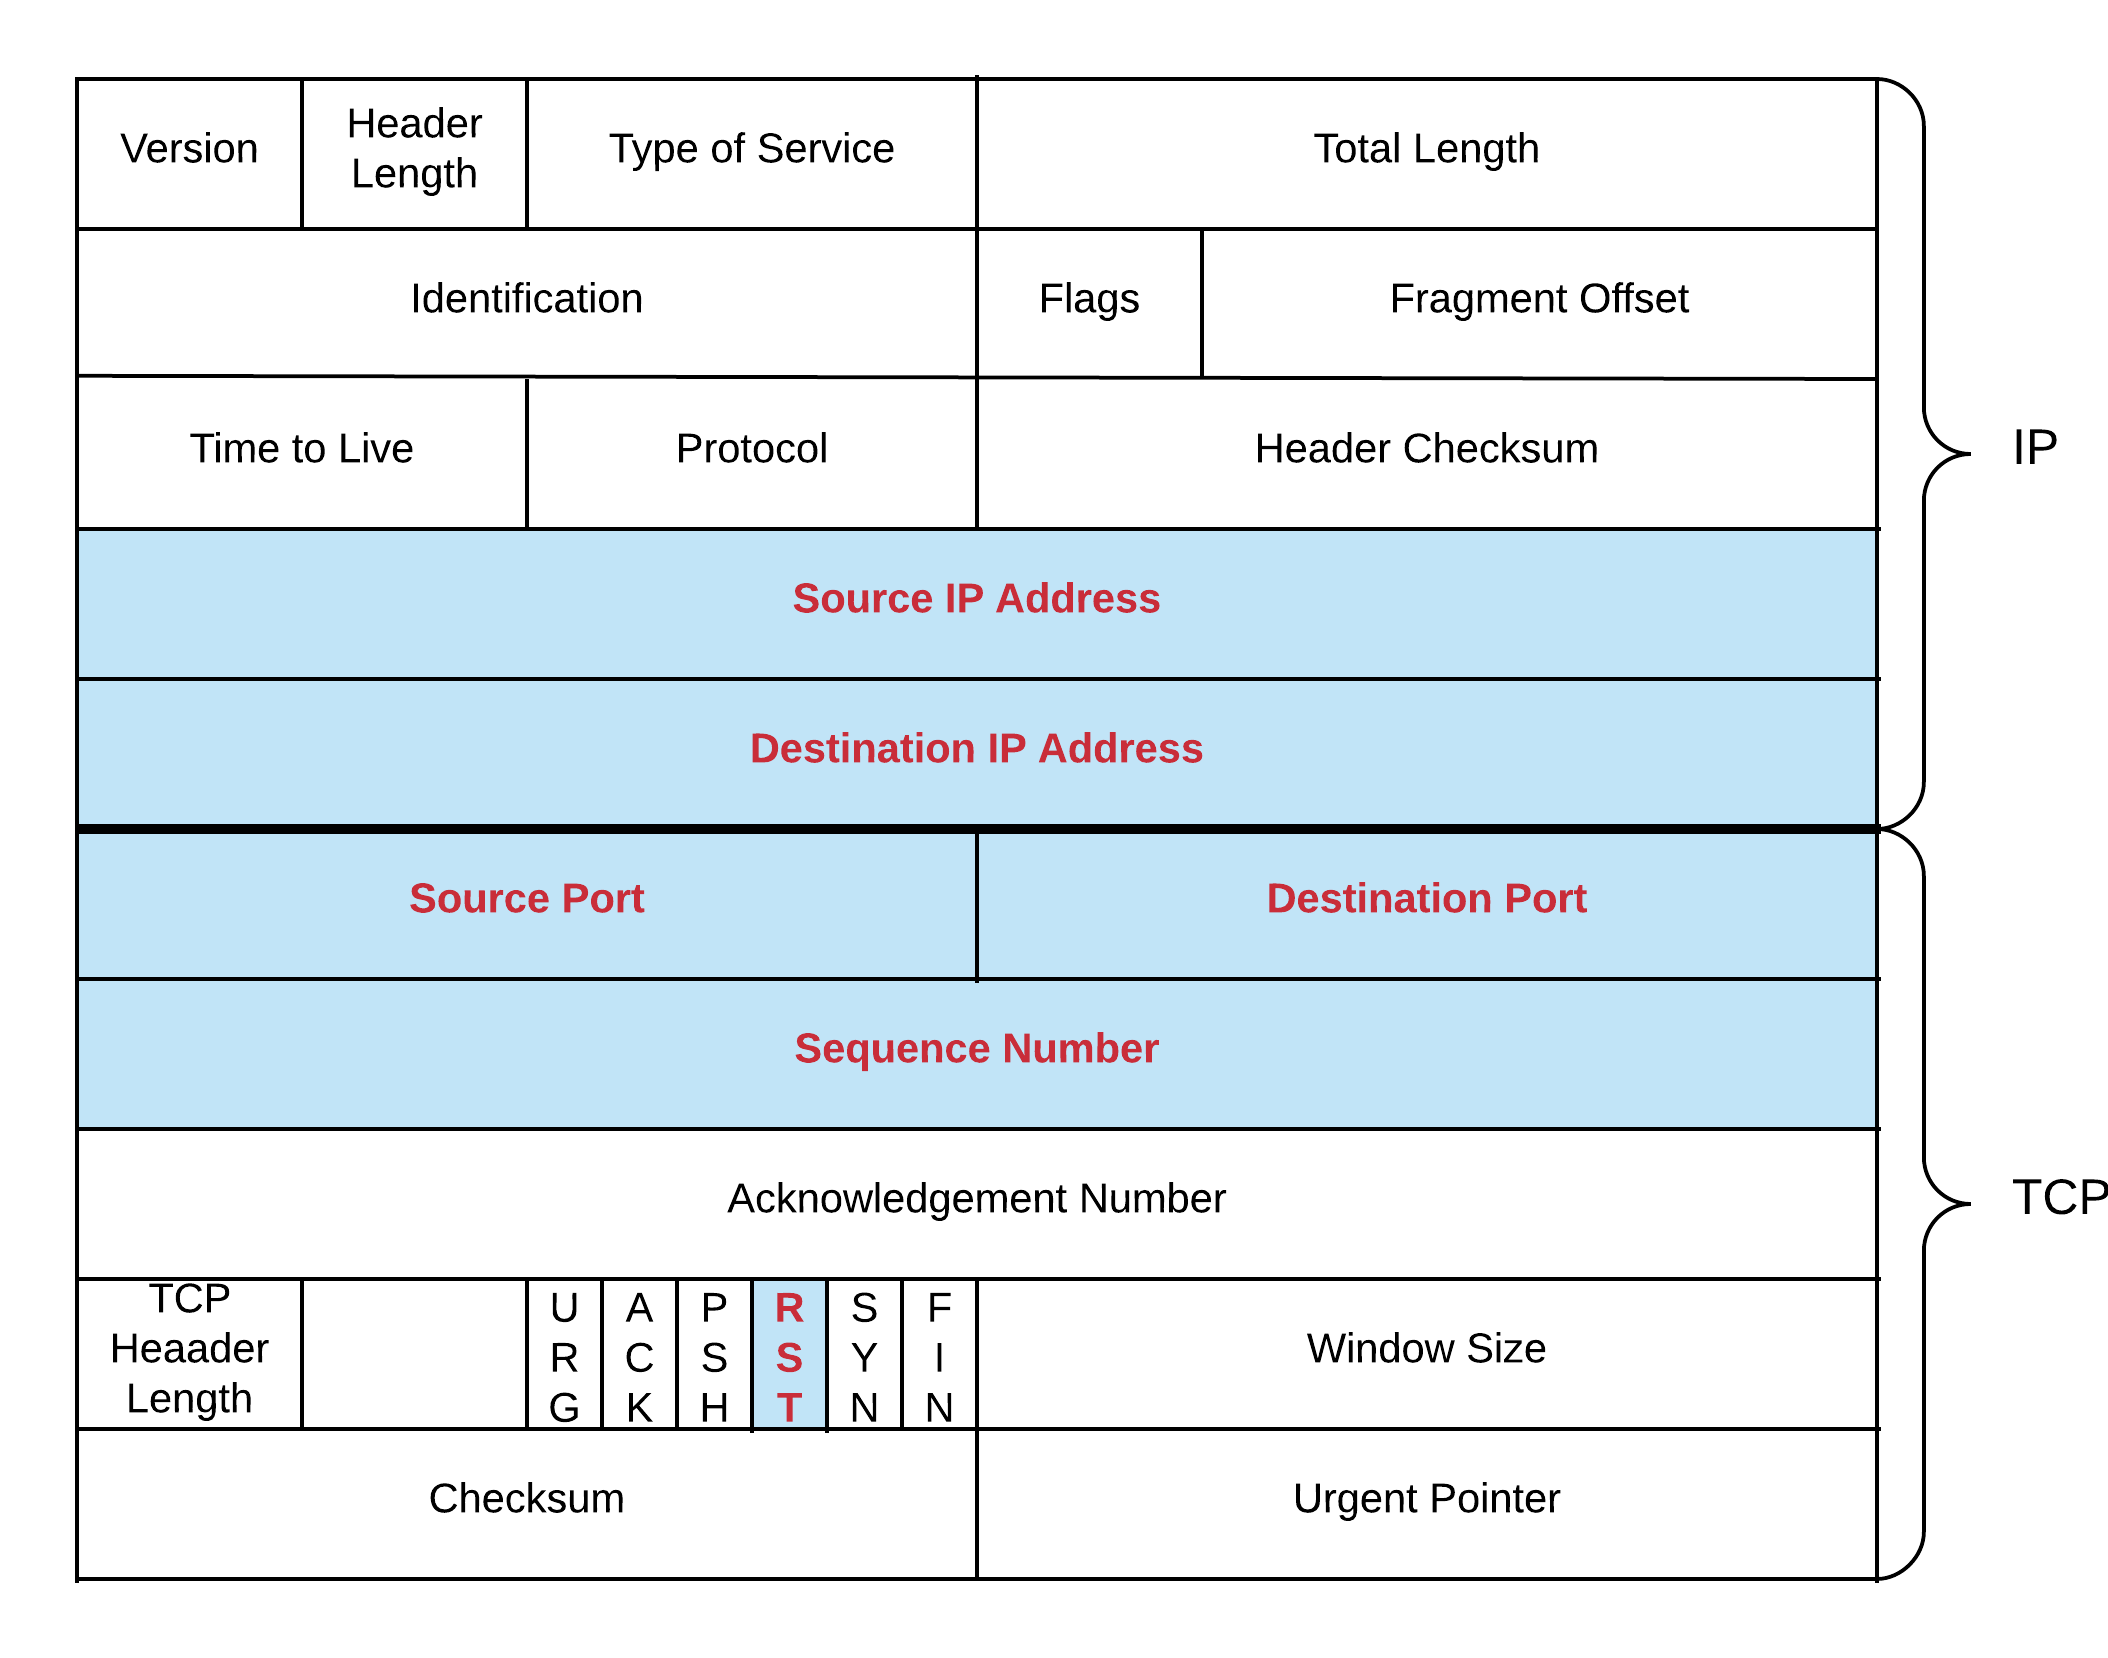
\includegraphics[width=.85\textwidth]{Pictures/TCP_IP_Packet.png}
    	\caption{Attack Packet Header} 
    	\label{fig:Attack_Packet}
    \end{figure}

    In figure \ref{fig:Attack_Packet}, we show the specific fields in the TCP/IP header that need to be handled in order to perform TCP reset attack. Here source IP will be the video streaming server's IP address, Destination IP will be victim's IP address, and the port numbers will be set correspondingly. Sequence number must be correctly discovered through sniffing. Finally RST bit must be set to 1. The other fields will be changed accordingly with the help of programming language libraries. Also payload to this header is not really important in this case as it is merely an RST packet.

\section{Available Tools}
    There are already a few available tools for many different network attacks. Among them \textbf{Netwox} is quite well known. To perform TCP reset attack from an Linux environment, the command is as follows:
    
    \subfile{Codes/Netwox.tex}
    
    Although being readily available, there is a major drawback of Netwox. For working correctly, we already know from Section \ref{sec:strategy} that sequence number of the forged packet must be within the victims window. Also port numbers must be set correctly. But sniffing is not possible with "pcap" API with packets from other devices on the network, which are connected through switch. As a result where Wireshark does not work, neither does Netwox 78 command. \\ 
    Tests on Wireshark are mentioned in Section \ref{apx:test_wireshark} where it can be seen in Figure \ref{fig:main2vm} that the guest OS cannot sniff packets from the host OS. Similarly Netwox is tested in a VM environment from the guest OS where pcap API does not work attacking the host OS. \\
    The result of the test can be seen in figure \ref{fig:netwox_test} where video in the browser of the host can still load the played video. So the attack failed.
    
    \begin{figure}
    	\centering
    	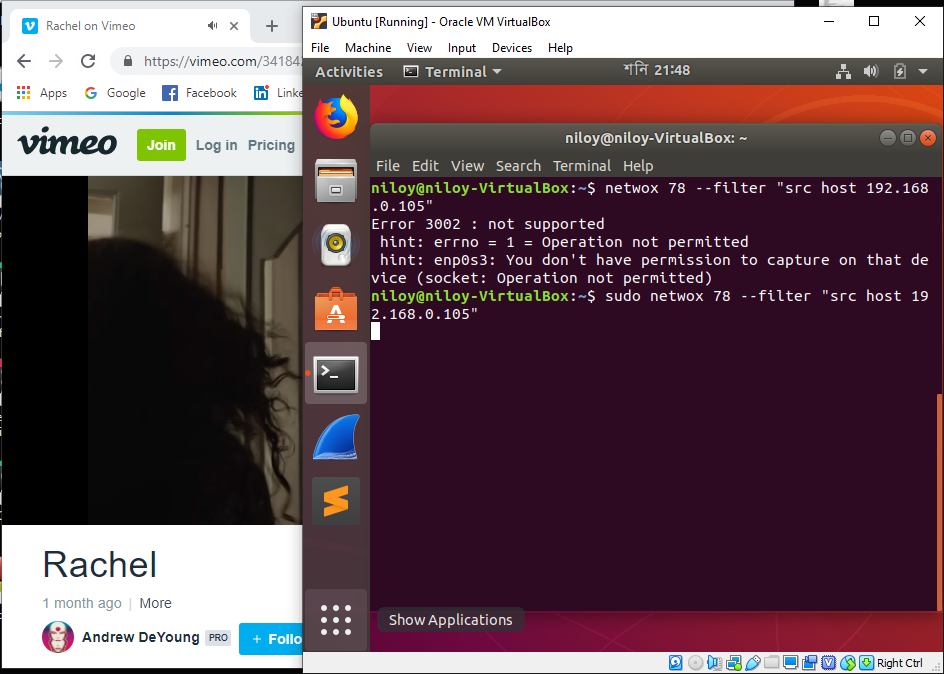
\includegraphics[width=.95\textwidth]{Pictures/Netwox_test.png}
    	\caption{Netwox Test} 
    	\label{fig:netwox_test}
    \end{figure}
    

\section{Video Streaming Server}
    Our target is to disrupt videos from any website that uses TCP connection. For implementation purpose, we will use the website \textbf{"Vimeo.com"} as video streaming server. \\
    Although YouTube is the most popular video streaming website, it uses UDP connection which is out of the scope of our attack tool. This choice of website is based on tests described in Section \ref{apx:test_server} where Wireshark is used to determine the transport layer protocol used by these websites.    

\section{Implementation Technology}
    \begin{description}
    
    \item[Language:] We are going to use \textbf{Python 3.7} for implementation purpose. One of the main reasons for choosing this language is that it has ample support for forging TCP packets and sending them to appropriate destination. 
    
    \item[Libraries:] First we need a library to sniff packets. We will use \textbf{libpcap} package for this purpose. Secondly, We will use \textbf{scapy} package for forging and sending packets. Both of these are from Python.
    
    \end{description}



\section{Implementation Environment}
    
    We will use \textbf{Oracle VM VirtualBox}  for implementation purpose. The tool will be implemented in 2 phases. Those are: 
    
    \begin{figure}
        \centering
        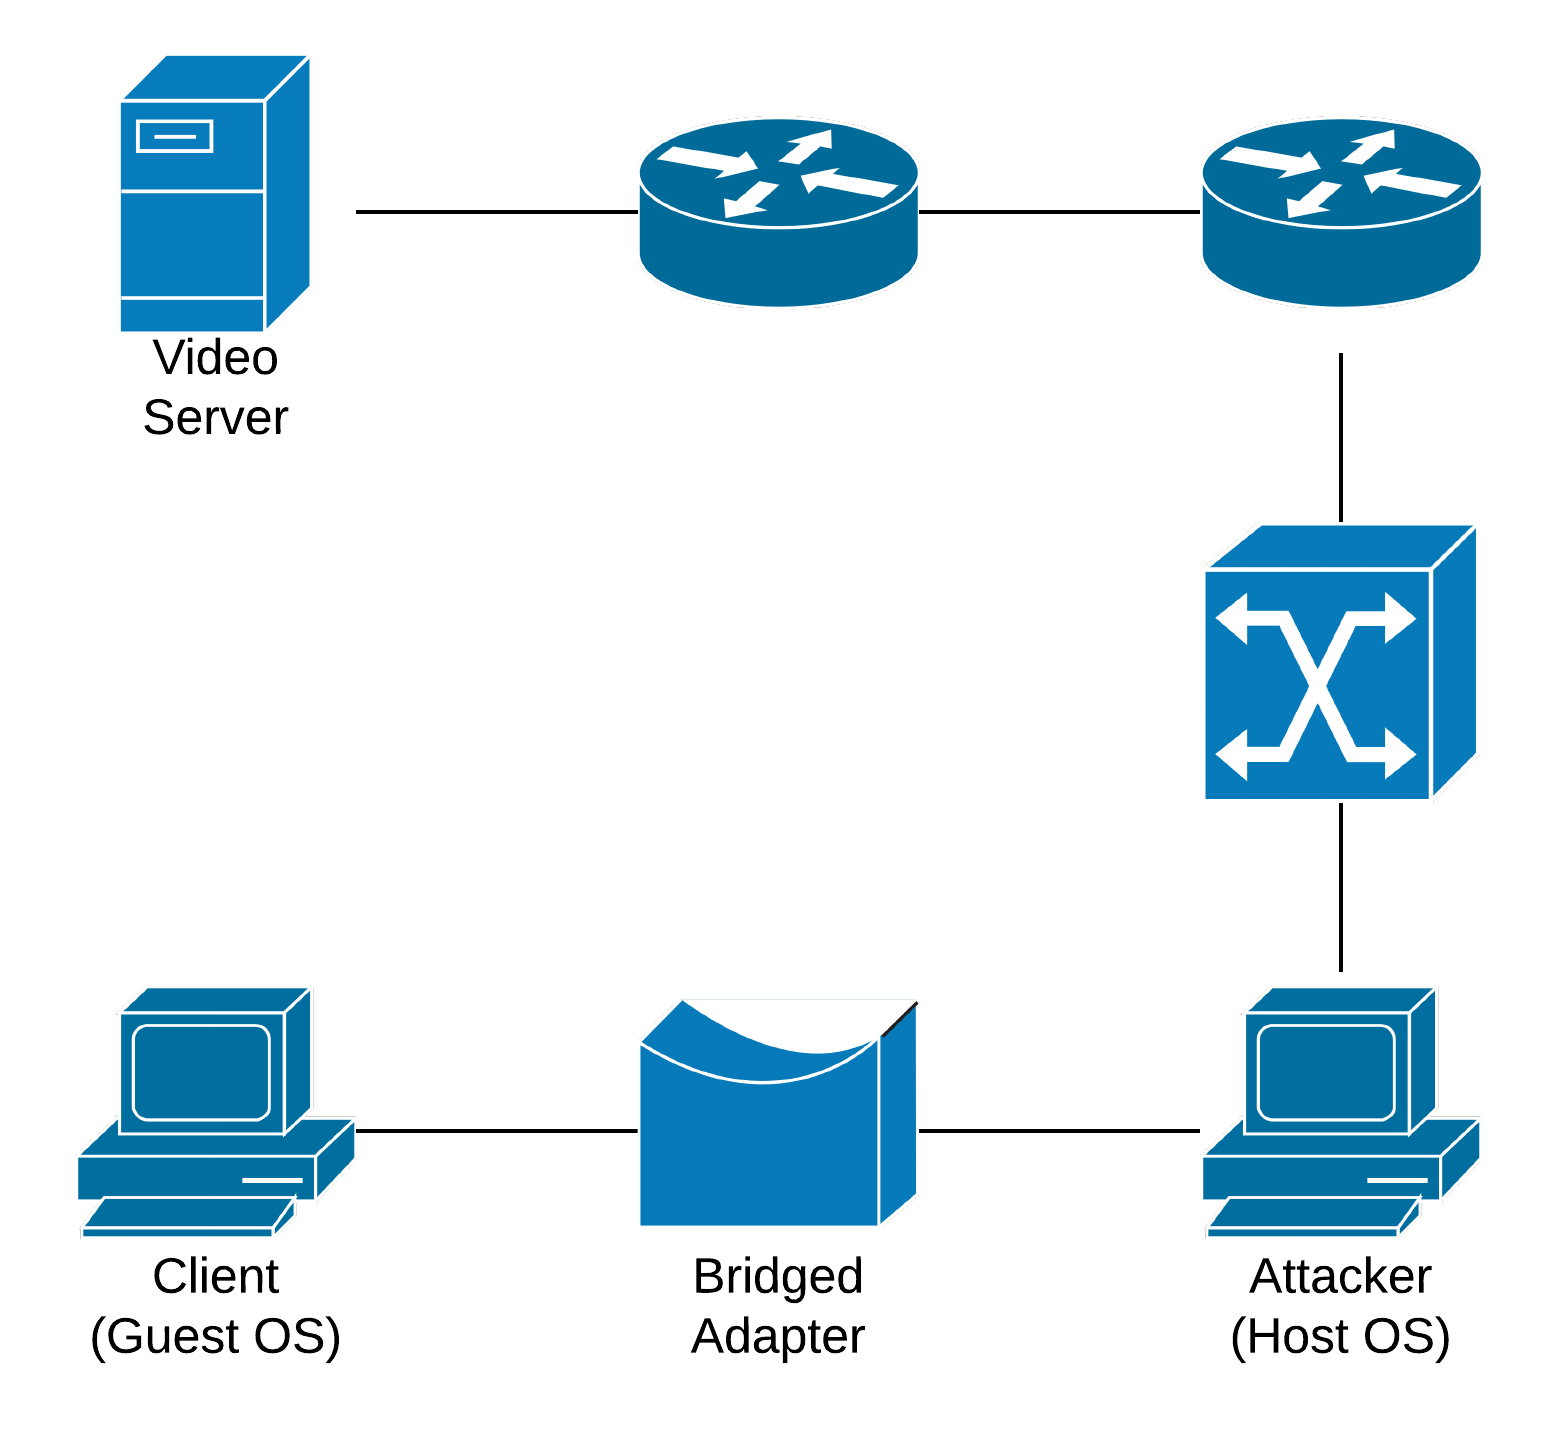
\includegraphics[width=.75\textwidth]{Pictures/TCP_RST_Topology_Implementation.png}
        \caption{Implementation Topology}
        \label{fig:topolgy_implement}
    \end{figure}
    
    
    \begin{enumerate}
      
      \item First we will implement the TCP reset attack part assuming that we can sniff packets of victim machine. As shown in Section \ref{apx:test_wireshark} (Figure \ref{fig:main2vm}), packets for guest OS can be sniffed from host OS. As TCP reset attack requires sniffing packets destined for other devices, we will use host OS as the attacker machine and guest os of the VirtualBox as victim machine for this part. This topology is shown in Figure \ref{fig:topolgy_implement} where guest OS is connected through bridged network adapter. Video streaming server is remotely situated in the network.
      
      \item In this phase, we will implement the part where we can sniff packets from different machines on the network. For this part we will flip the roles of attacker and victim of Figure \ref{fig:topolgy_implement} where we will try to sniff packets in guest OS. As shown in Section \ref{apx:test_wireshark} (Figure \ref{fig:vm2main}), normally guest OS cannot sniff host OS' packets, but if we can enrich the tool with additional attacking mechanisms of \textbf{Man in the Middle} and take advantage of \textbf{ARP cache} of the network switch, it will become a very unique tool as compared to other available tools at this moment.
      
      \end{enumerate}
    
    
\section{Target Environment}
    \label{sec:target_environment}
    \begin{figure}[!h]
        \centering
        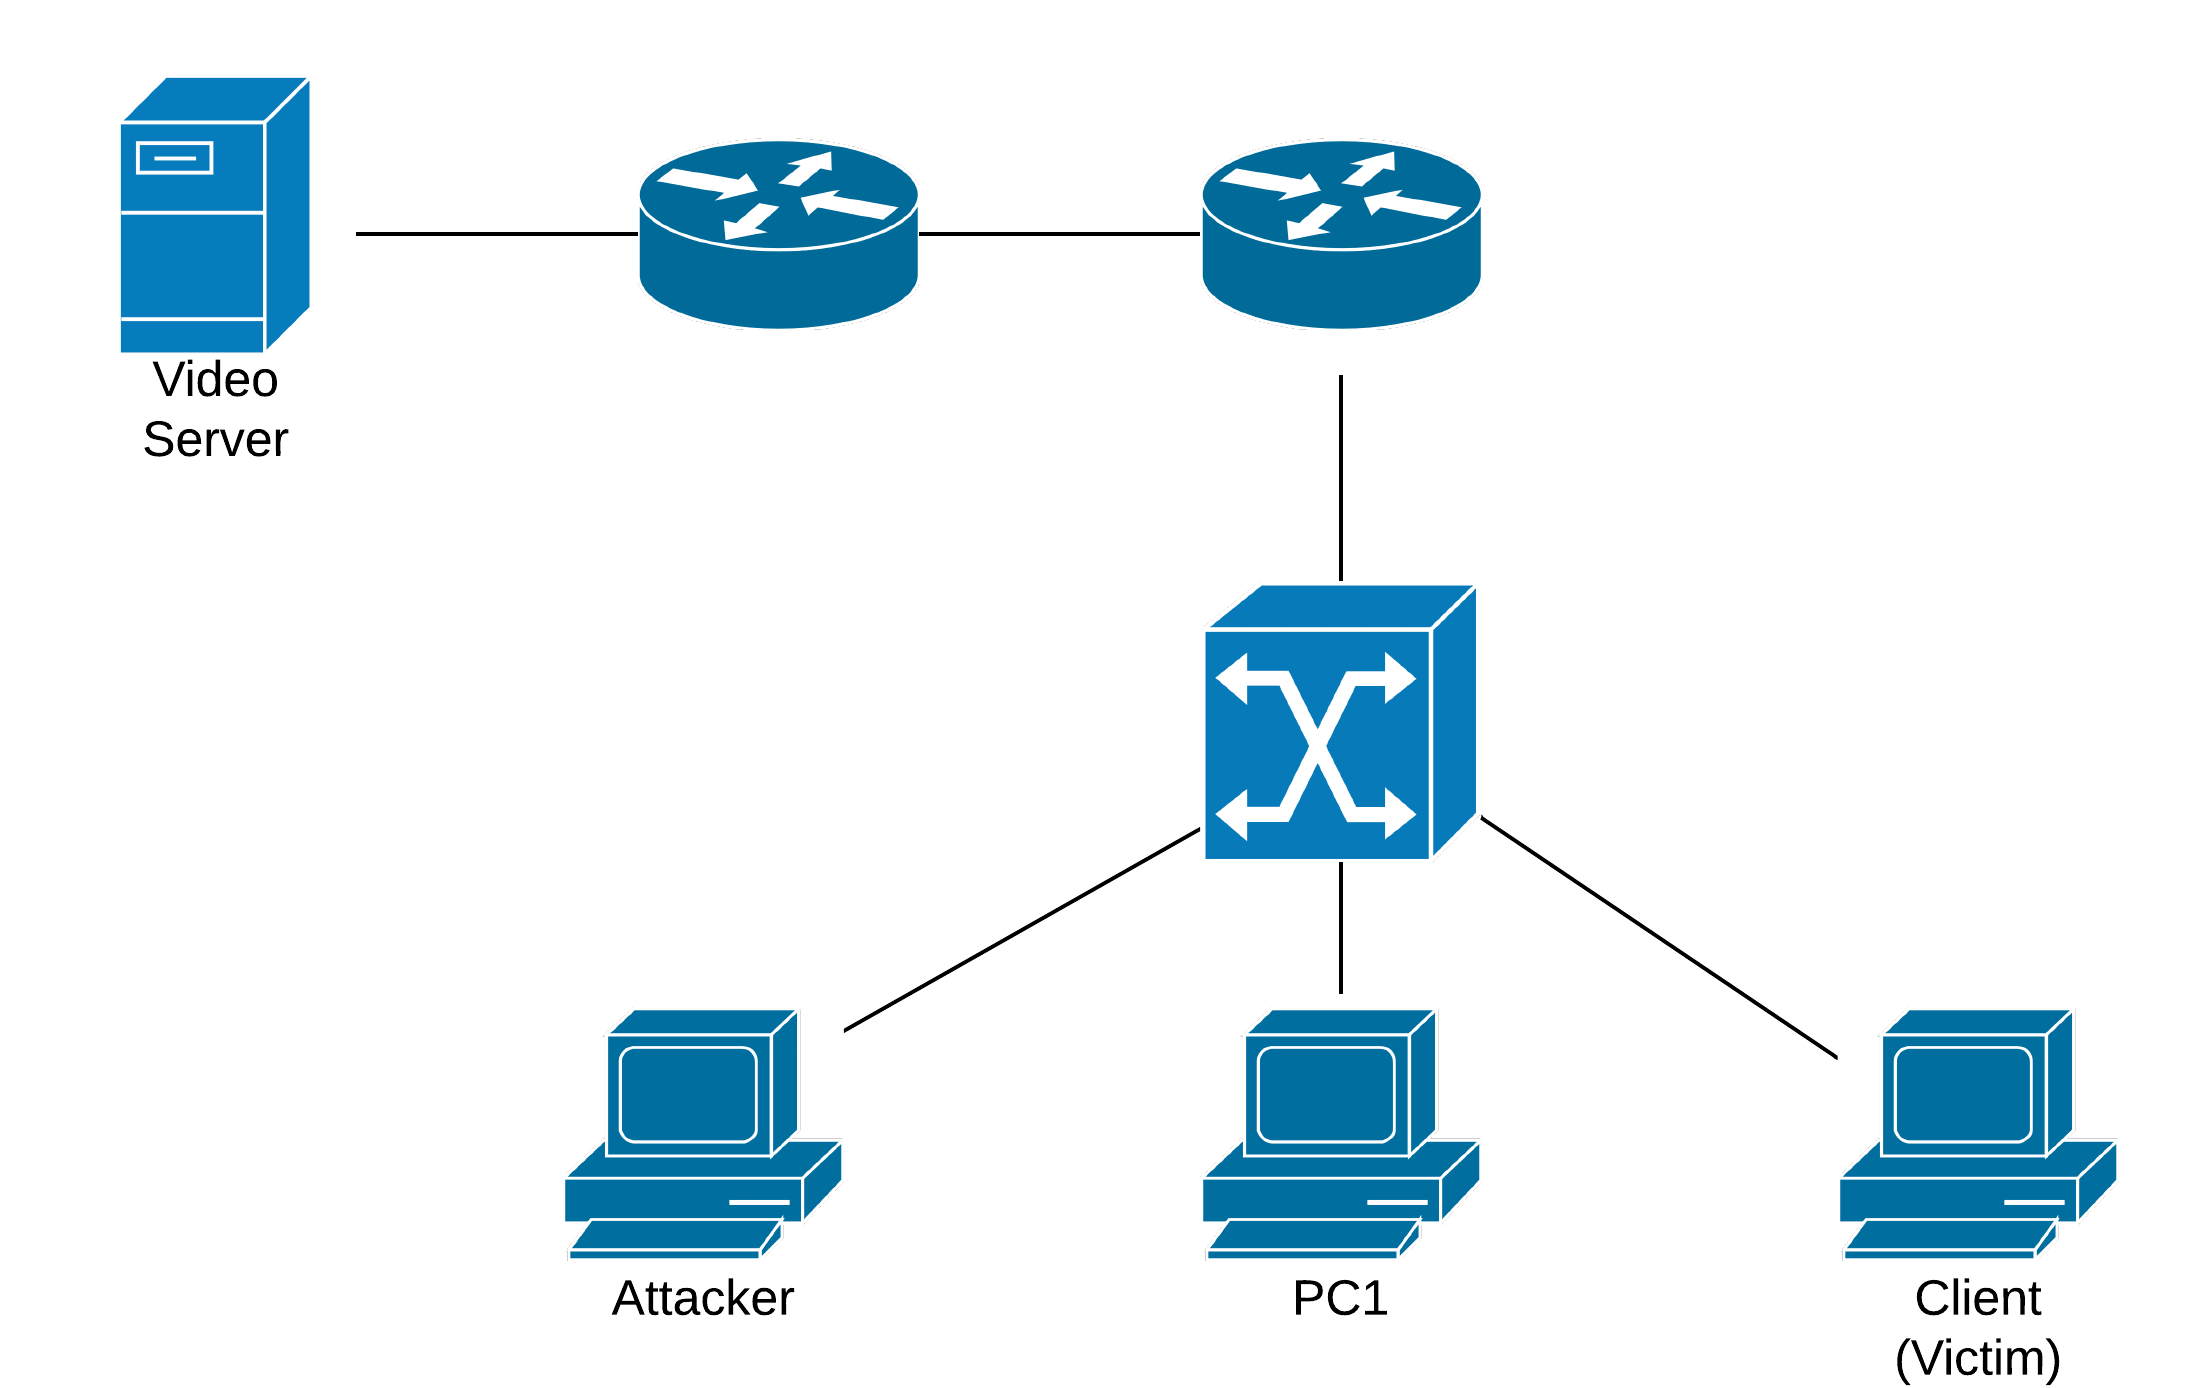
\includegraphics[width=.95\textwidth]{Pictures/TCP_RST_Topology_Easy.png}
        \caption{Target Topology}
        \label{fig:topology}
    \end{figure}
    
     As our target environment, we have designed a topology as shown in figure \ref{fig:topology}. Here the attacker and the victim are in the same subnet and the server is in a remote network. Without the loss of generality there can be more switches or routers in the network, and more hosts connected to the switch. This type of topology is carefully chosen as we need to sniff packets destined to the victim machine to gather information about source IP, TCP port numbers and sequence number in order to successfully perform a TCP reset attack.

   


\section{Justification}
    When the victim machine in our design receives the RST packet, it does not have any idea about the packet's actual origin. If we correctly specify IP addresses, port numbers and sequence number, it can perfectly mimic its identity as an original. So the victim machine has no option other than to terminate its TCP connection. The main challenge in this approach is to forge a packet with correct sequence number and to send it quickly within the victim's window. If we can do that, it can be inferred from above discussion that our TCP reset attack will be successful.

\section{Defence Mechanism}

\section{Appendix A: Testing Video Straming Server Connection}
    \label{apx:test_server}
    We have performed some tests to determine which website can be used for implementing our attack tool. If we can perform correctly for a website with TCP connection, it can be generalized for any website using the same.
    
    \subsection{YouTube}
    The test failed. YouTube does not use TCP connection. Rather it uses UDP connection. It is shown in Figure \ref{fig:youtube} with the help of Wireshark.
    \begin{figure}
        \centering
        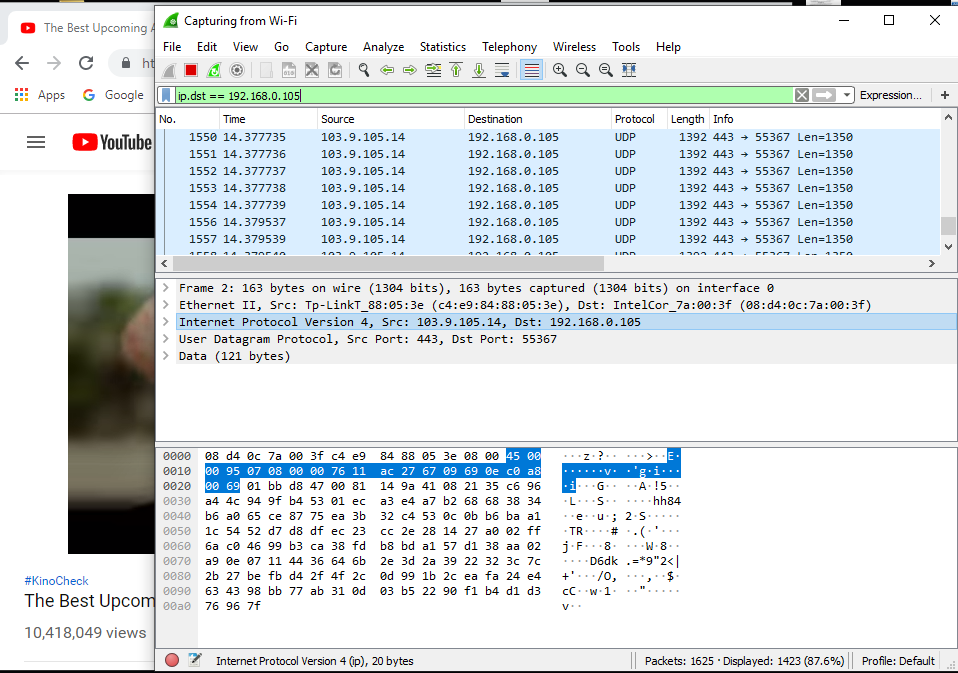
\includegraphics[width=.95\textwidth]{Pictures/Youtube_test.png}
        \caption{YouTube Connection}
        \label{fig:youtube}
    \end{figure}
    
    
    \subsection{Vimeo}
    The test successful. Vimeo does indeed use TCP connection. It is shown in Figure \ref{fig:vimeo} with the help of Wireshark. So it can be used in our implementation.
    \begin{figure}
        \centering
        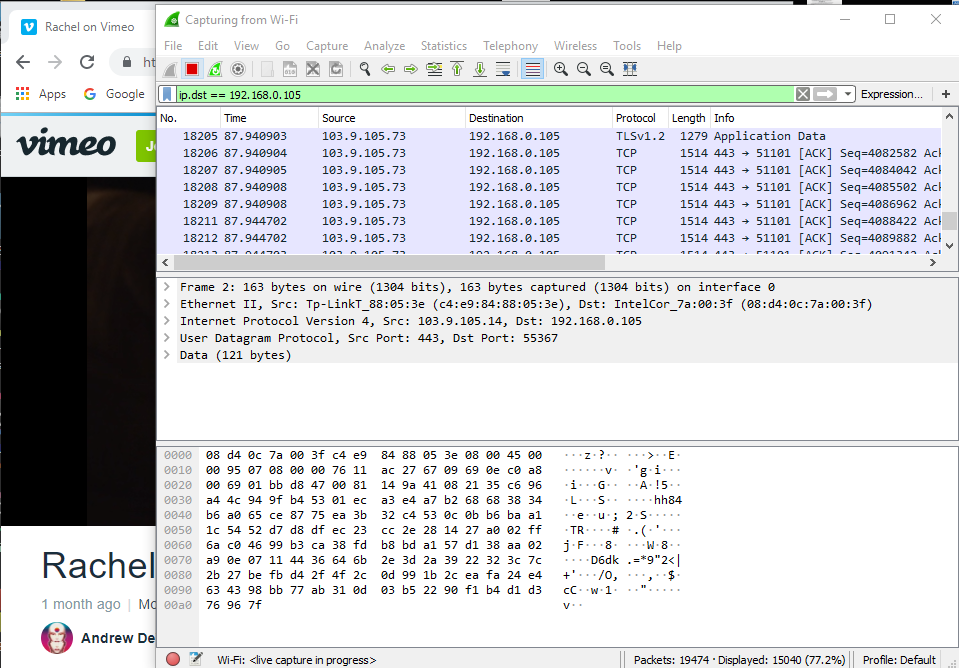
\includegraphics[width=.95\textwidth]{Pictures/Vimeo_test.png}
        \caption{Vimeo Connection}
        \label{fig:vimeo}
    \end{figure}
    

\section{Appendix B: Testing Sniffing with VM}
    \label{apx:test_wireshark}
    We have performed test with \textbf{Oracle VM VirtualBox} to see how Wireshark behaves in this environment. Here the host OS has IP address: 172.20.56.3 and the 2 guest OS' have IP addresses: 172.20.56.50 and 172.20.56.54.
    
    \subsection{Guest Sniffing Host's Packet}
        The test failed. The guest OS cannot sniff packets of the host OS. It is shown in Figure \ref{fig:vm2main}.
        \begin{figure}
            \centering
            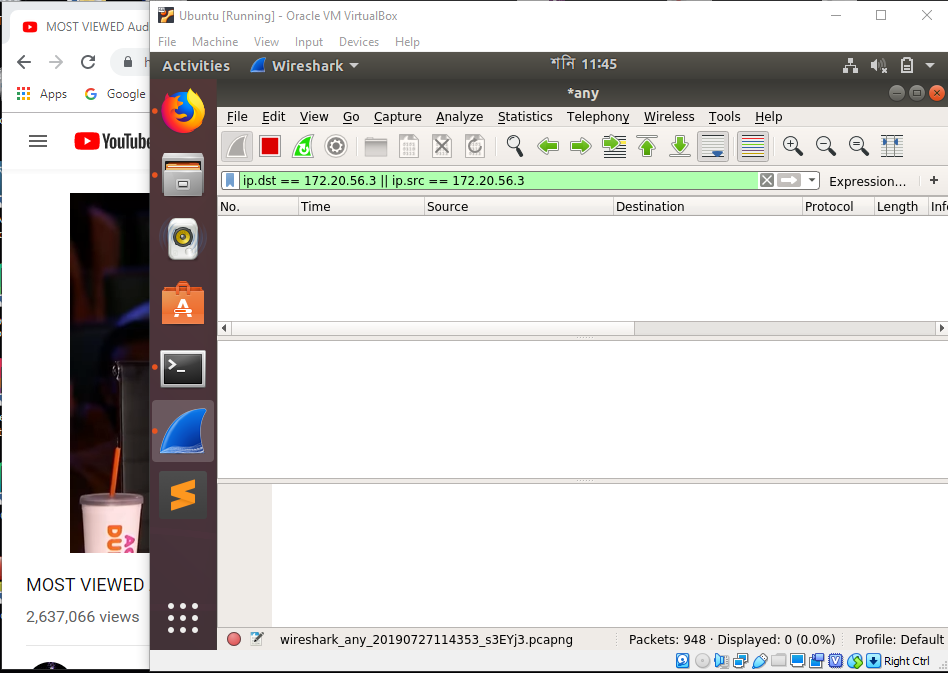
\includegraphics[width=.95\textwidth]{Pictures/VM1_to_main.png}
            \caption{Guest Sniffing Host's Packet}
            \label{fig:vm2main}
        \end{figure}
    
    \subsection{Guest Sniffing Another Guest's Packet}
        The test failed. The guest OS cannot sniff packets of other guest's OS. It is shown in Figure \ref{fig:vm2vm}.
        \begin{figure}
            \centering
            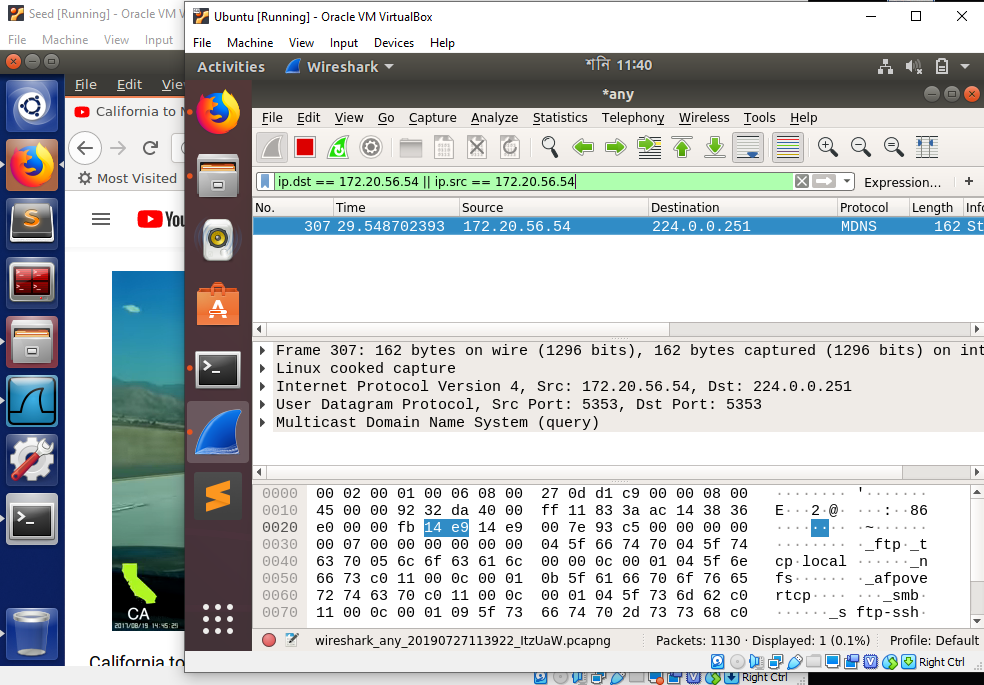
\includegraphics[width=.95\textwidth]{Pictures/VM1_to_VM2.png}
            \caption{Guest Sniffing Another Guest's Packet}
            \label{fig:vm2vm}
        \end{figure}    
    
    \subsection{Host Sniffing Guest's Packet}
        The test is successful. The host OS can sniff packets of the guest's OS. It is shown in Figure \ref{fig:main2vm}.
        \begin{figure}
            \centering
            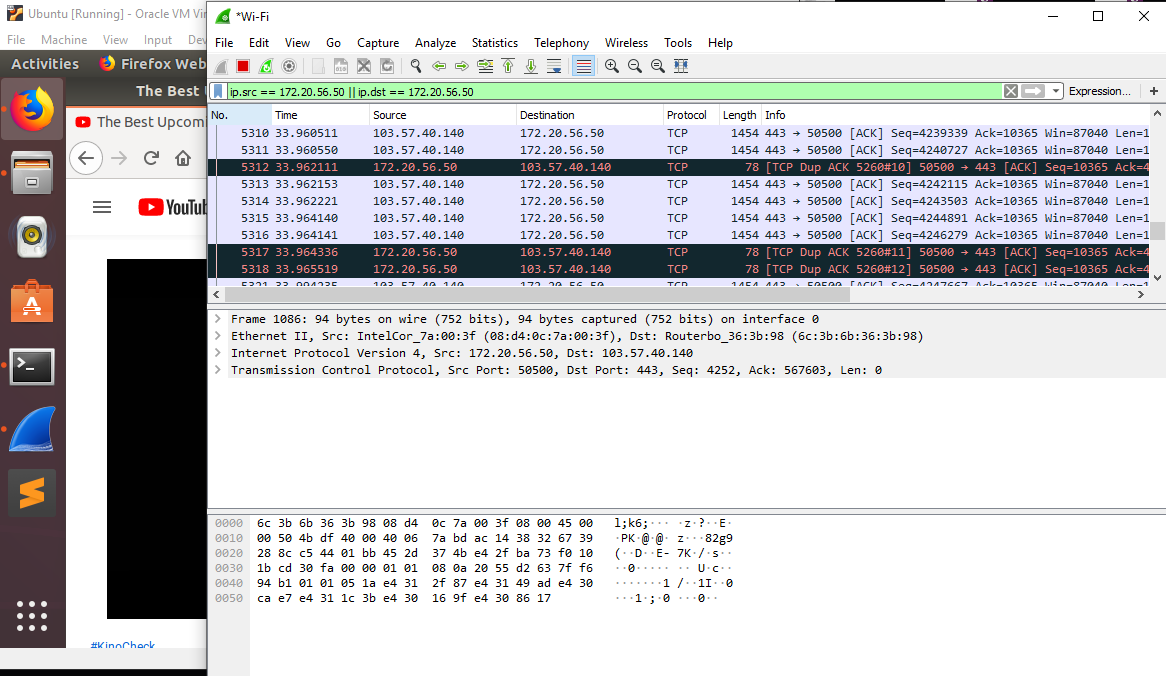
\includegraphics[width=.95\textwidth]{Pictures/Main_to_VM1.png}
            \caption{Host Sniffing Guest's Packet}
            \label{fig:main2vm}
        \end{figure}

\end{document}
